\documentclass[tikz,border=10pt]{standalone}
\usepackage{tikz}
\usetikzlibrary{shapes,arrows,positioning,calc}

% Use sans-serif font
\renewcommand{\familydefault}{\sfdefault}

\begin{document}

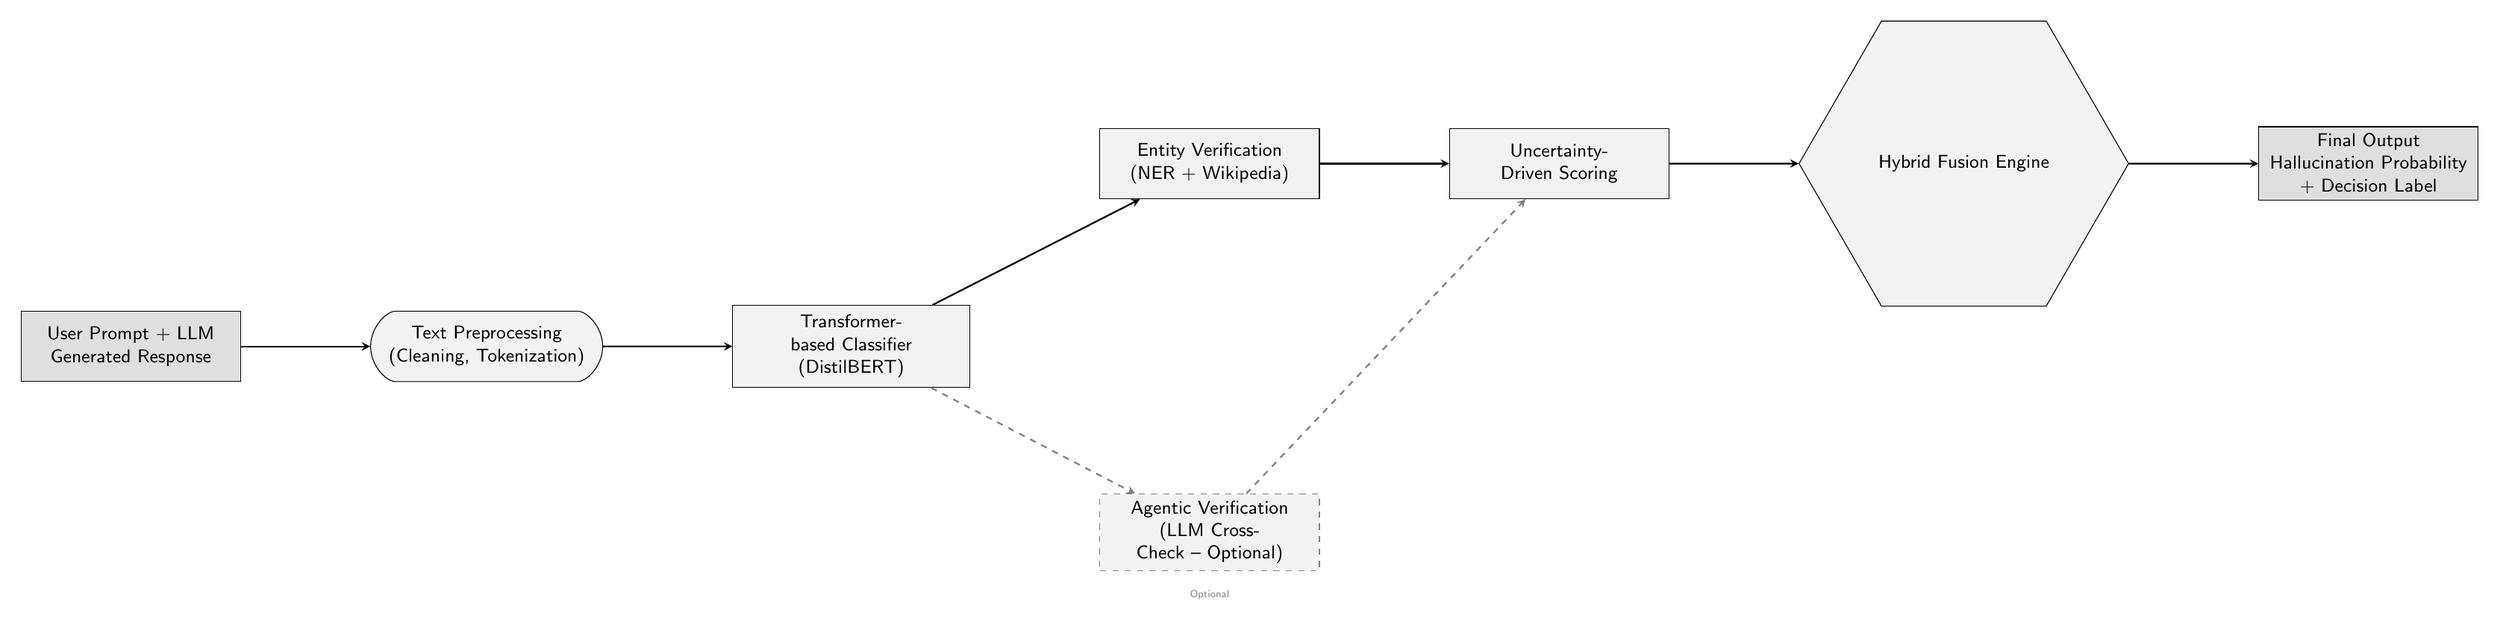
\begin{tikzpicture}[
    % Node styles
    input/.style={rectangle, draw=black, fill=gray!25, text width=3.5cm, 
                  text centered, minimum height=1.2cm, font=\small},
    preprocess/.style={rounded rectangle, rounded corners=5pt, draw=black, 
                      fill=gray!10, text width=3.5cm, text centered, 
                      minimum height=1.2cm, font=\small},
    primary/.style={rectangle, draw=black, fill=gray!10, text width=3.8cm, 
                   text centered, minimum height=1.4cm, font=\small},
    block/.style={rectangle, draw=black, fill=gray!10, text width=3.5cm, 
                  text centered, minimum height=1.2cm, font=\small},
    optional/.style={rectangle, draw=black!50, fill=gray!10, text width=3.5cm, 
                    text centered, minimum height=1.2cm, font=\small, dashed},
    uncertainty/.style={rectangle, draw=black, fill=gray!10, text width=3.5cm, 
                       text centered, minimum height=1.2cm, font=\small},
    fusion/.style={regular polygon, regular polygon sides=6, draw=black, 
                   fill=gray!10, text width=3.2cm, text centered, 
                   minimum height=1.4cm, font=\small},
    output/.style={rectangle, draw=black, fill=gray!25, text width=3.5cm, 
                   text centered, minimum height=1.2cm, font=\small},
    arrow/.style={thick,->,>=stealth,black},
    optionalarrow/.style={thick,->,>=stealth,black!50,dashed},
    label/.style={font=\tiny, text=black!50}
]

% 1. Input
\node[input] (input) at (0,0) {
    User Prompt + LLM Generated Response
};

% 2. Preprocessing
\node[preprocess, right=2.2cm of input] (preprocess) {
    Text Preprocessing\\
    (Cleaning, Tokenization)
};

% 3. Transformer-based Classifier (Primary block)
\node[primary, right=2.2cm of preprocess] (transformer) {
    Transformer-based Classifier\\
    (DistilBERT)
};

% 4. Entity Verification (Top branch - solid)
\node[block, above right=1.8cm and 2.2cm of transformer] (entity) {
    Entity Verification\\
    (NER + Wikipedia)
};

% 5. Agentic Verification (Bottom branch - optional, dashed)
\node[optional, below right=1.8cm and 2.2cm of transformer] (agentic) {
    Agentic Verification\\
    (LLM Cross-Check -- Optional)
};

% Optional label
\node[label, below=0.2cm of agentic] {Optional};

% 6. Uncertainty-Driven Scoring (convergence point)
\node[uncertainty, right=2.2cm of entity] (uncertainty) {
    Uncertainty-Driven Scoring
};

% 7. Hybrid Fusion Engine (Hexagon)
\node[fusion, right=2.2cm of uncertainty] (fusion) {
    Hybrid Fusion Engine
};

% 8. Final Output
\node[output, right=2.2cm of fusion] (output) {
    Final Output\\
    Hallucination Probability\\
    + Decision Label
};

% Main flow arrows (solid)
\draw[arrow] (input) -- (preprocess);
\draw[arrow] (preprocess) -- (transformer);

% Split into two branches from Transformer
\draw[arrow] (transformer) -- (entity);  % Top branch - solid
\draw[optionalarrow] (transformer) -- (agentic);  % Bottom branch - dashed

% Converge into Uncertainty-Driven Scoring
\draw[arrow] (entity) -- (uncertainty);  % Top branch - solid
\draw[optionalarrow] (agentic) -- (uncertainty);  % Bottom branch - dashed

% Continue main flow
\draw[arrow] (uncertainty) -- (fusion);
\draw[arrow] (fusion) -- (output);

\end{tikzpicture}

\end{document}

